% Chapter Template

\chapter{Gestió i desenvolupament} % Main chapter title

\label{GestioIDesenvolupament} % Change X to a consecutive number; for referencing this chapter elsewhere, use \ref{ChapterX}

Abans d'entrar en els detalls del projecte, necessitem definir sota quins criteris i quines pràctiques realitzarem la gestió i el desenvolupament del projecte.

%----------------------------------------------------------------------------------------
%	SECTION 1
%----------------------------------------------------------------------------------------

\section{Metodologia de desenvolupament}

Les necessitats i requisits específics del projecte aniran fortament relacionades amb la recerca i l’avenç del propi transcurs del projecte. Si bé els objectius específics queden clars, les tasques a desenvolupar aniran evolucionant dinàmicament. Per aquesta raó, en aquest cas serà adequat seguir una metodologia de desenvolupament àgil. I, en concret, es seguirà una simplificació de la metodologia Kanban. \\

En base als requisits establerts inicialment durant la planificació del projecte, i al llarg del seu transcurs, s’aniran generant una sèrie de tasques que s’afegiran a un backlog o to-do list; és a dir, el conjunt de tasques amb la mínima granularitat que aporti valor al projecte com a producte entregable. D’acord a les necessitats, s’aplicarà una priorització, i aquestes tasques s’aniran afegint com a tasques realitzant o en progrés. Conforme aquestes tasques es completin, s’afegiran al llistat de tasques realitzades o done, mantenint així un control dels requisits que s’estan satisfent i el seu grau de completesa. \\

\begin{figure}
\centering
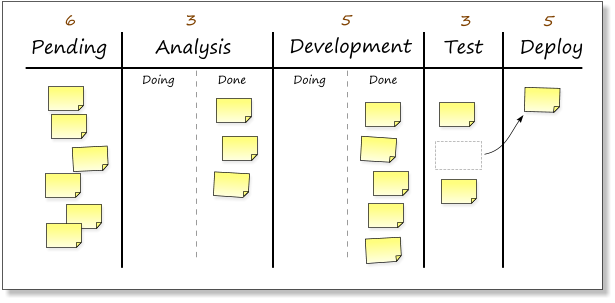
\includegraphics[width=8cm]{Figures/Figure3}
\decoRule
\caption[Simplificació de la metodologia Kanban]{Simplificació de la metodologia Kanban}
\label{fig:Figura3}
\end{figure}

Per garantir la integritat del sistema, cadascuna d’aquestes tasques serà desenvolupada fora de l’entorn de producció, en un entorn (o branca) separats. D’aquesta manera, el desenvolupament no afectarà al producte provisional generat en cada moment del desenvolupament del projecte. I, alhora, permetrà fer un seguiment més exacte de l’estat de cada tasca o funcionalitat a implementar. \\

S’ha considerat millor opció a, per exemple, alternatives àgils com Scrum, degut a diversos factors. P.e., a Kanban les entregues o releases són constants, i no acotades temporalment. Considerarem més important, per tant, la metodologia basada en el producte final. \\

%-----------------------------------
%	SUBSECTION 1
%-----------------------------------
\section{Recursos}

Per definir les necessitats de recursos per satisfer la realització del projecte, els classificarem segons el següent criteri: recursos \textbf{humans}, recursos \textbf{materials} i recursos \textbf{software}.\\

\noindent \textbf{\large Recursos humans}\\

\noindent Pel domini de nostre projecte, basat en 1 desenvolupador principal i 2 gestors de projecte (1 director + 1 co-director), considerarem les seves hores de treball com recursos humans. Estimarem, i considerant els següents aspectes:

\begin{itemize}
\item El TFG es correspon a 18 ECTS (3 crèdits ECTS GEP + 15 crèdits ECTS TFG)
\item 1 ECTS = 25-30 hores de treball
\item Durada aproximada TFG = 22 setmanes
\end{itemize}

Podem estimar, per tant, pel cas del desenvolupador (alumne) una dedicació d’unes \textbf{24 hores} a la setmana. Pel cas dels gestors, farem una estimació aproximada de \textbf{50 hores} en total per part dels dos rols, com a tasques de suport.\\

\noindent \textbf{\large Recursos materials}\\

\noindent Els recursos materials per aquest projecte són relativament senzills. Bàsicament:

\begin{itemize}
\item \textbf{Portàtil Lenovo G-50}. Màquina principal amb la qual es durà a terme el projecte
\item \textbf{Materials d'impressió}. Necessaris per documentació, impressió de memòria, etc.
\end{itemize}

\noindent \textbf{\large Recursos software}\\

\noindent Tot i que aquests es discutiran amb més detall al capítol \textit{5. Eines de desenvolupament}, podem identificar inicialment la necessitat d'alguns recursos software principals, tals com:

\begin{itemize}
\item \textbf{Gestor de versions}. El codi (emmagatzemament, desenvolupament i evolució) requereix un control i manteniment, motiu pel qual s'estableix com a necessitat una eina d'aquest tipus
\item \textbf{IDE}. És necessari l'ús d'un entorn de desenvolupament integrat per desenvolupar el projecte, dissenyar l'arquitectura, realitzar la implementació, configurar l'entorn, etc.
\item \textbf{Sistema de compilació automàtic}. Necessari per gestionar la compilació i les dependències dels projectes.
\item \textbf{Framework desenvolupament web}. Segons les necessitats que es defineixin al llarg del projecte, es triarà una tecnologia específica per desenvolupar el dashboard definit com a requisit al projecte.
\end{itemize}

Les opcions triades per suplir les necessitats d'aquests recursos i altres recursos software identificats com a necessaris es plantejaran més endavant.

\section{Planificació temporal}

Segons les necessitats d’aquest projecte i les seves característiques, classificarem el desenvolupament en 4 fases: la planificació, el disseny, la implementació, i la documentació i entrega del projecte. 

\subsection{Descripció de fases}

\noindent \textbf{\large Planificació}\\

\noindent En primer lloc cal una fase inicial o fase de planificació. L’objectiu principal d’aquesta fase del projecte és definir els aspectes bàsics que definiran la naturalesa del projecte: els objectius, la metodologia de treball, el desenvolupament, els requisits, la planificació, etc. És a dir, tot allò relacionat amb l’establiment de les premisses sobre les quals ens basarem per desenvolupar el nostre projecte. \\

Aquesta fase del projecte va fortament lligada al desenvolupament del curs GEP, juntament amb altres activitats. En definitiva, les tasques a realitzar són les següents:

\begin{itemize}
\item \textbf{P1.} Investigació i recerca en quant al monitoratge i l’adaptabilitat de sistemes software.
\item \textbf{P2.} Definir l’abast i el context del projecte. 
\item \textbf{P3.} Definir les fases i tasques del projecte, així com una planificació temporal de desenvolupament.
\item \textbf{P4.} Preparar una gestió econòmica i una anàlisi de sostenibilitat.
\item \textbf{P5.} Establir els requisits i necessitats d’acord a l’especialitat d’Enginyeria del Software.
\item \textbf{P6.} Definir les eines de desenvolupament i els llenguatges amb els que treballar i implementar el sistema i el dashboard.
\item \textbf{P7.} Definir els casos d'ús per validar i implementar el sistema.
\end{itemize}

\noindent \textbf{\large Disseny}\\

Conforme la fase de planificació avanci, podrem començar a realitzar el disseny del nostre sistema des d’un punt de vista de requisits i també arquitectònic (en referència a arquitectura del software). És a dir: l’objectiu d’aquesta fase és passar dels conceptes i objectius definits a la planificació a un “mapa” o “esquema” que serveixi de guia pel desenvolupament del projecte (subjecte, per descomptat, a possibles canvis i adaptacions al llarg del desenvolupament). \\

Principalment, les tasques a incloure en aquesta fase són:

\begin{itemize}
\item \textbf{D1.} Definir els entorns de configuració sota els quals es desenvoluparà el projecte
\item \textbf{D2.} Dissenyar l’arquitectura software del sistema de monitoratge i dels monitors
\item \textbf{D3.} Definir els criteris d’adaptabilitat amb els quals es dotarà al sistema
\item \textbf{D4.} Configurar un entorn de configuració d’acord amb els criteris definits
\item \textbf{D5.} Documentar els avanços referents a aquesta fase (memòria)
\end{itemize}

\noindent \textbf{\large Implementació}\\

\noindent Aquesta fase tindrà la major càrrega de feina de tot el projecte. Partirà d’uns criteris i objectius ben definits i estructurats a partir de les anteriors fases. Les tasques es correspondran principalment a totes aquelles tasques d’implementació i de testing del nostre sistema. \\

Per tant, identificarem com a tasques:

\begin{itemize}
\item \textbf{I1.} Implementació de l’arquitectura genèrica del sistema de monitoratge.
\item \textbf{I2.} Implementació del sistema de monitors.
\item \textbf{I3.} Implementació del sistema d'adaptabilitat.
\item \textbf{I4.} Integració dels sistemes.
\item \textbf{I5.} Implementació d’un dashboard que permeti visualitzar l’activitat del sistema
\item \textbf{I6.} Generació de documentació referent al desenvolupament i la implementació (documentació d’APIs, README per desplegar el sistema, manual d’usuari del dashboard, etc.)
\item \textbf{I7.} Ampliació del sistema (afegir monitors, ampliar dashboard) en funció de les necessitats i/o de la disponibilitat temporal
\item \textbf{I8.} Redacció i ampliació de la memòria
\end{itemize}

\noindent \textbf{\large Fase final}\\

\noindent Finalment, identificarem una darrera fase del projecte que servirà de cloenda per preparar l’entrega i defensa final de la feina realitzada, així com tancar possibles tasques pendents i assegurar el correcte funcionament del sistema i la generació d’un producte final adequat. \\

Les tasques principals seran:

\begin{itemize}
\item \textbf{F1.} Testing de les funcionalitats del sistema
\item \textbf{F2.} Comprovació de la satisfacció dels objectius i requisits
\item \textbf{F3.} Finalització i revisió de la memòria
\item \textbf{F4.} Preparació de la defensa final
\end{itemize}

\subsection{Previsió d'alternatives i pla d'acció}

La planificació temporal i de tasques plantejada, així com el consum de recursos, contempla un desenvolupament del treball regular i sense imprevistos. Tot i així, hem de considerar alternatives al desenvolupament fruït d’imprevistos, desviacions o altres factors no contemplats dins de la normalitat. Identificarem, per tant, les possibles següents desviacions:

\begin{itemize}
\item \textbf{Increment del nº d’hores necessàries.} Aquest problema pot ser derivat per diverses causes (inhabilitació temporal del desenvolupador, dificultats tècniques en el desenvolupament, etc.). Això pot provocar, per una banda, una necessitat de més hores, i per altra banda, més dedicació per unitat de temps.
\subitem \textbf{Pla d’acció.} La tasca corresponent a la implementació del dashboard serà adaptada en funció de l’estat del projecte arribat al moment. És a dir: al tractar-se d’un requisit molt flexible en quant a la seva complexitat (podem aspirar a un dashboard molt complet i multifuncional, o bé establir els requisits mínims per satisfer els criteris d’acceptació del TFG), podem permetre’ns retallar hores d’aquesta tarda, prioritzant aspectes crucials (com p.e. la implementació dels monitors). 
\item \textbf{Avaria en el hardware.} És possible que durant el desenvolupament del projecte el hardware utilitzat (en aquest cas, el portàtil Lenovo G-50) pateixi alguna avaria. Al tractar-se de la principal eina de desenvolupament, això pot afectar als terminis de desenvolupament.
\subitem \textbf{Pla d’acció.} Dues mesures complementàries: per una banda, en tot moment es mantindran diverses còpies de seguretat de tots els artefactes generats (documentació, software, entorns de configuració…) per garantir-ne la recuperabilitat; per altra banda, disposarem d’un entorn de treball alternatiu (un sistema operatiu instal·lat a un disc dur extern) on podrem seguir el desenvolupament del nostre projecte paral·lelament mentre l’avaria es soluciona.
\item \textbf{Canvis en els requisits del projecte.} Podem suposar que el desenvolupament pràctic del projecte ens durà a concloure nous canvis necessaris en quant als requisits prèviament establerts.
\subitem \textbf{Pla d’acció.} En primer lloc, sotmetre a constant revisió el projecte per tal d’evitar al màxim que es produeixi un canvi de requisits significatiu. Per fer-ho, constantment es revisaran requisits, nivell de viabilitat, i satisfacció envers els terminis establerts. Si, per contra, es produeix un canvi significatiu inevitable, el nº d’hores total del projecte (aproximats) permet un petit increment fruit d’aquesta desviació, per tal de garantir que la resta de tasques es duen a terme correctament.
\end{itemize}

%-----------------------------------
%	SUBSECTION 2
%-----------------------------------

\section{Viabilitat}

Un dels principals objectius del Treball de Final de Grau és plasmar la capacitat de l'estudiant de generar, mitjançant els coneixements obtinguts, un producte o projecte real, amb una utilitat i uns objectius aplicables al nostre entorn. Per aquest motiu, i com estudiants, cal assumir la responsabilitat del projecte i estudiar-ne la seva viabilitat en dos sentits. Per una banda, la seva viabilitat econòmica, mitjançant una estimació pressupostària dels costos del projecte en un àmbit professional. Per altra banda, el seu impacte econòmic, social i ambiental des d'un punt de vista de sostenibilitat.

%----------------------------------------------------------------------------------------
%	SECTION 2
%----------------------------------------------------------------------------------------

\subsection{Estimació pressupostària}

Per simplificar al màxim l’estudi dels costos i, alhora, clarificar i estudiar-ne la justificació, procedirem a identificar i estimar els diferents costos associats al projecte segons el seu tipus.\\

\noindent \textbf{\large Despeses directes}\\

\noindent Entraran dins la classificació de despeses directes aquelles despeses derivades directament de la realització d’activitats previstes pel desenvolupament del projecte. Per una major precisió, relacionarem directament les activitats definides a l’anterior entregable amb els costos directes.  \\

\begin{table}[htb]
\centering
\label{PressupostActivitats}
\resizebox{\textwidth}{!}{%
\begin{tabular}{lrrrrr}
\hline \textbf{ACTIVITAT}                           & {\color[HTML]{000000} \textbf{HORES TOTALS}} & {\color[HTML]{000000} \textbf{DEVELOPER}} & {\color[HTML]{000000} \textbf{DIRECTOR}} & {\color[HTML]{000000} \textbf{CODIRECTOR}} & {\color[HTML]{000000} \textbf{COST TOTAL}} \\ \hline
{\color[HTML]{000000} \textbf{Planificació}} & {\color[HTML]{000000} \textbf{149}}          & {\color[HTML]{000000} \textbf{125}}            & {\color[HTML]{000000} \textbf{12}}       & {\color[HTML]{000000} \textbf{12}}         & {\color[HTML]{000000} \textbf{2475,00\euro}} \\
\hline
Abast i context                              & 30                                           & 25                                             & 2,5                                      & 2,5                                        & 500,00\euro                                        \\
Planificació                                 & 12                                           & 10                                             & 1                                        & 1                                          & 200,00\euro                                        \\
Gestió econòmica i sostenibilitat            & 12                                           & 10                                             & 1                                        & 1                                          & 200,00\euro                                        \\
Requisits d'especialitat                     & 12                                           & 10                                             & 1                                        & 1                                          & 200,00\euro                                        \\
Recerca de la temàtica                       & 38                                           & 30                                             & 4                                        & 4                                          & 650,00\euro                                        \\
Eines de desenvolupament                     & 20                                           & 20                                             & 0                                        & 0                                          & 300,00\euro                                        \\
Definir casos d'ús                           & 25                                           & 20                                             & 2,5                                      & 2,5                                        & 425,00\euro                                        \\
\hline
\textbf{Disseny}                             & \textbf{102}                                 & \textbf{88}                                    & \textbf{4}                               & \textbf{10}                                & \textbf{1670,00\euro}                              \\
\hline
Entorn de configuració                       & 15                                           & 15                                             & 0                                        & 0                                          & 225,00\euro                                        \\
Arquitectura software                        & 32                                           & 25                                             & 2                                        & 5                                          & 550,00\euro                                        \\
Criteris d'autoadaptabilitat                 & 25                                           & 20                                             & 2                                        & 3                                          & 425,00\euro                                        \\
Integració continuada                        & 20                                           & 18                                             & 0                                        & 2                                          & 320,00\euro                                       \\
Documentació memòria                         & 10                                           & 10                                             & 0                                        & 0                                          & 150,00\euro                                        \\
\hline
\textbf{Implementació}                       & \textbf{203}                                 & \textbf{186}                                   & \textbf{0}                               & \textbf{17}                                & \textbf{3215,00\euro}                              \\
\hline
Implementació arquitectura genèrica                       & 30                                           & 26                                             & 0                                        & 4                                          & 490,00\euro                                        \\
Implementació monitors                       & 70                                           & 65                                             & 0                                        & 5                                          & 1100,00\euro                                        \\
Implementació sistema d'adaptabilitat                      & 50                                           & 45                                             &0                                        & 5                                          & 800,00\euro                                        \\
Integració sistemes                      & 20                                           & 20                                             & 0                                        & 0                                          & 300,00\euro                                        \\
Implementació dashboard                      & 33                                           & 30                                             & 0                                        & 3                                          & 525,00\euro                                        \\
Documentació de components                   & 15                                           & 15                                             & 0                                        & 0                                          & 225,00\euro                                        \\
Ampliació del sistema                        & 15                                           & 15                                             & 0                                        & 0                                          & 225,00\euro                                        \\
Documentació memòria                         & 10                                           & 10                                             & 0                                        & 0                                          & 150,00\euro                                        \\
\hline
\textbf{Fase final}                          & \textbf{85}                                  & \textbf{75}                                    & \textbf{4}                               & \textbf{6}                                 & \textbf{1375,00\euro}                              \\
\hline
Finalització tasques                         & 10                                           & 10                                             & 0                                        & 0                                          & 150,00\euro                                        \\
Testing                                      & 19                                           & 15                                             & 2                                        & 2                                          & 325,00\euro                                        \\
Comprovació satisfacció                      & 14                                           & 10                                             & 2                                        & 2                                          & 250,00\euro                                        \\
FInalització memòria                         & 25                                           & 25                                             & 0                                        & 0                                          & 375,00\euro                                        \\
Preparació defensa final                     & 17                                           & 15                                             & 0                                        & 2                                          & 275,00\euro                                        \\
\hline
\textbf{Total}                               & \textbf{539}                                 & \textbf{474}                                   & \textbf{20}                              & \textbf{45}                                & \textbf{8735,00\euro}       \\
\hline                      
\end{tabular}}
\caption{Costos directes}
\end{table}

Per aquest cas, farem les següents assumpcions:

\begin{itemize}
\item En el projecte intervindran 3 agents: el desenvolupador (alumne), i dos gestors de projectes (director i codirector). La principal diferència entre el director i codirector, per aquest cas, serà la involucració de cadascun en el desenvolupament del projecte segons la fase (el director tindrà major pes durant la fase inicial, mentre que el codirector donarà més suport al desenvolupament).
\item L’estimació del cost serà de 12\euro /hora pel desenvolupador i 25\euro /hora pels gestors del projecte, en base a la informació actual que podem trobar referent a aquest aspecte pels rols de programador junior i gestor de projecte a portals com InfoJobs.
\end{itemize}

Per cada activitat estimarem un nº d’hores total i un grau d’implicació de cada rol. Les unitats corresponen a hores pel nº d’hores totals i de cada rol, i a \euro pel cost total.\\

\noindent \textbf{\large Despeses indirectes i amortitzacions}\\

\noindent Considerarem les següents despeses indirectes i amortitzacions:

\begin{itemize}
\item \textbf{Impressions a paper}. Considerarem 150 fulls / memòria, a 3 memòries a entregar per la defensa final + 1 de provisional; com a afegit, 200 fulls per articles, documentació… fan un total de 800 fulls.
\item \textbf{Electricitat}. Cost i consum en base a referències de característiques de portàtil i preu estàndard de companyies elèctriques.
\item \textbf{Amortització}. portàtil Lenovo G-50. Cost en base a compra; percentatge d’amortització en base a les hores útils de vida aproximada i les hores de rendiment esperades de programació, documentació, etc.
\item \textbf{Software}. El desenvolupament serà basat en software lliure i, per tant, sense despesa addicional, però el considerarem com a part del pressupost per possibles desviacions.
\end{itemize}

\begin{table}[htb]
\centering
\label{PressupostIndirectes}
\resizebox{\textwidth}{!}{%
\begin{tabular}{lrrrrr}
\hline \textbf{CONCEPTE}                           & {\color[HTML]{000000} \textbf{COST UNITARI}} & {\color[HTML]{000000} \textbf{UNITATS}} & {\color[HTML]{000000} \textbf{COST}}\\ 
\hline
Impressions a paper                              & 0,03\euro /full                                           & 800 fulls                                             & 24,00\euro\\
Electricitat                                 & 0,20\euro /kWh                                           & 225 kWh                                           & 45,00\euro\\
Amortització portàtil Lenovo G-50            & 450,00\euro /portàtil                                           & 0,15 (amortitzat)                                             & 67,50\euro   \\
Software                     & 0,00\euro /mes                                           & 5 mesos                                             & 0,00\euro \\                                       
\hline
\textbf{Total}                               &                              &                                & \textbf{136,50\euro}       \\
\hline                      
\end{tabular}}
\caption{Costos indirectes i amortitzacions}
\end{table}


\noindent \textbf{\large Contingències}\\

\noindent Afegirem, en base als costos directes i indirectes prèviament desglosats, un 15\% sobre el total en concepte de contingències.

\begin{table}[htb]
\centering
\label{PressupostContingencies}
%\resizebox{\textwidth}{!}{%
\begin{tabular}{lrrrrr}
\hline \textbf{CONCEPTE}                           & {\color[HTML]{000000} \textbf{COST BASE}} & {\color[HTML]{000000} \textbf{\% CONTINGÈNCIES}} & {\color[HTML]{000000} \textbf{TOTAL}}\\ 
\hline
Costos directes                             & 8735,00\euro /full                                           & 15                                             & 1310,25\euro\\
Costos indirectes                                 & 136,50\euro /kWh                                           & 15                                           & 20,475\euro\\
\hline
\textbf{Total}                               &                              &                                & \textbf{1330,725\euro}       \\
\hline                      
\end{tabular}%}
\caption{Contingències}
\end{table}

\noindent \textbf{\large Imprevistos}\\

\noindent Identificarem 2 imprevistos en base a la planificació:

\begin{itemize}
\item \textbf{Prolongació de les hores / ampliació del termini}. Contemplarem la possibilitat de requerir més temps de l’estimat per acabar el projecte, considerant una desviació de fins a 50 hores (que podríem considerar la dedicació aproximada de dues setmanes a mitja jornada). Considerarem una probabilitat raonable del 20%.
\item \textbf{Avaria de hardware}. Problemes en l’ús del material hardware (en aquest cas, exclusivament el portàtil). Considerarem una probabilitat més remota, del 5\%, i el pitjor dels casos, que equivaldria a la substitució total del cost del portàtil.
\end{itemize}

\begin{table}[htb]
\centering
\label{PressupostImprevistos}
\resizebox{\textwidth}{!}{%
\begin{tabular}{lrrrrr}
\hline \textbf{CONCEPTE}                           &  \textbf{COST UNITARI} &  \textbf{\ UNITATS} & \textbf{COST TOTAL} & \textbf{\% PROBABILITAT} &  \textbf{TOTAL} \\
\hline
Ampliació del termini                             & 12,00\euro /hora                                           & 50 hores                                             & 600,00\euro & 20 & 120,00\euro \\
Avaria del hardware                                 & 450,00\euro /ordinador & 1 ordinador                                           & 450,00\euro & 5 & 22,50\euro \\
\hline
\textbf{Total}                               &                              &                                & & & \textbf{142,50\euro}       \\
\hline                      
\end{tabular}}
\caption{Imprevistos}
\end{table}

\noindent \textbf{\large Pressupost global}\\

\noindent Un cop valorat costos indirectes, costos indirectes i amortitzacions, contingències i possibles imprevistos, podem donar una versió completa de l’estimació pressupostària per la realització del projecte.

\begin{table}[htb]
\centering
\label{PressupostGlobal}
%\resizebox{\textwidth}{!}
\caption{Resum global del pressupost}
\end{table}

Per tant, el pressupost final és de \textbf{9867,475\euro}.

\subsection{Control de gestió}

El pressupost exposat ja inclou com a part de la partida destinada una part generada per imprevistos i desviacions amb possibilitats de produir-se i que pretenen precisament realitzar un control i manteniment de la gestió i evolució del projecte i els recursos (veure apartats 2.1.3. i 2.1.4.).\\

Tot i així, podem considerar oportú establir uns mecanismes, o tasques específiques, dedicades al control periòdic que permetin fer un seguiment de l’activitat de gestió de projecte i, per tant, no només preveure de forma teòrica aspectes com desviacions pressupostàries, sinó detectar al llarg de l’evolució del projecte quan això succeeixi.\\

Per fer-ho es proposa realitzar un control de desviacions durant la transició de fases; és a dir, treballarem amb un model de plantilla que ens calculi una sèrie de desviacions (en funció de diversos criteris), que al finalitzar cada fase ens permeti obtenir un feedback objectiu i ràpid de possibles desviacions respecte al pressupost inicial.\\

Per fer-ho, i basant-nos en la bibliografia utilitzada a GEP, farem servir els següents indicadors:

\begin{itemize}
\item \textbf{Desviament de mà d’obra en preu} = (cost estimat - cost real) * consum hores real
\item \textbf{Desviament en la realització d’una tasca en consum} = (consum estimat - consum real) * cost real
\item \textbf{Desviament total en la realització de tasques} = cost total estimat tasca - cost total real tasca
\item \textbf{Desviament total de despeses fixes} = total costos fixes pressupostat - total costos fixes real
\end{itemize}

Considerarem aquests 4 indicadors, ja que ens seran els més útils per detectar desviacions, p.e., en quant a la realització de les activitats descrites al Gantt, en termes tant de dedicació en quantitat d’hores total com per tasca, i també en aspectes com despeses fixes (p.e. amortitzacions). Mitjançant la comprovació d’aquests indicadors, podrem veure el grau de desviament i actuar en conseqüència segons les necessitats. 

\subsection{Sostenibilitat econòmica, social i ambiental}

Procedim a fer un anàlisi de les 3 dimensions de la sostenibilitat en referència a aquest projecte, per posteriorment avaluar fent servir la matriu de sostenibilitat el grau de satisfacció d’aquest àmbit en funció dels criteris establerts.\\

\noindent \textbf{\large Dimensió econòmica}\\

\noindent La dimensió econòmica està satisfactòriament treballada gràcies al pressupost prèviament exposat, basat en dades objectives i específiques (p.e., activitats reals a realitzar durant el projecte), que inclou despeses materials i humanes. Aquests costos i temps de dedicació inclouen aspectes crítics tals com possibles desviacions i imprevistos, i una assignació proporcional dels recursos assignats a la rellevància de cada tasca. Es tracta d’un projecte realitzat amb el cost mínim, però suficient (tenint en compte sempre que és necessari afegir extres per desviacions), garantint la seva satisfacció però sense despeses innecessàries, el que garanteix la seva viabilitat econòmica.\\

\noindent \textbf{\large Dimensió social}\\

\noindent L’objectiu principal del treball és aprofundir en el control de qualitat i monitoritatge de sistemes software mitjançant el desenvolupament de software lliure reaprofitable. Tal i com vam veure a l’entregable 1 (a l’apartat Estat de l’art), existeix marge d’investigació i treball en aquest àmbit, i l’àmplia gama de serveis software poden extreure un cert benefici en base als avenços (o si més no, la recerca i síntesi) que aquest projecte pugui aportar. Des del punt de vista dels desenvolupadors (usuaris reals d’aquest projecte, ja que seran els que l’utilitzaran), aportem noves eines i facilitem criteris d’autoadaptabilitat per monitors de control de qualitat. També, però, tindrà conseqüències en els usuaris dels sistemes monitorats, ja que la recol·lecció de dades d’aquests està orientada a la millora de la qualitat dels serveis oferts per aquests sistemes. Aquest és un aspecte que cada vegada requereix més profunditat, motiu pel qual podem considerar l’existència d’una necessitat dins el mercat actual. Podem considerar que no existeixen col·lectius afectats negativament.\\

\noindent \textbf{\large Dimensió ambiental}\\

\noindent Els recursos plantejats tant pel desenvolupament del projecte com el consum necessari per la seva vida útil són mínims, i inclouen únicament aquells derivats del manteniment d’un sistema software. No existirà contaminació destacada més allà de la generada pel consum d’electricitat del dispositiu portàtil a utilitzar pel desenvolupament del projecte o la impressió de papers (que es limitarà al mínim necessari). Es tracta, a més, d’un projecte que té per objectiu ser reaprofitat per tercers projectes (plantejant estructures, arquitectures, monitors, etc. reaprofitables).\\

\noindent \textbf{\large Matriu de sostenibilitat}\\

\noindent En base als anteriors criteris establerts, assignarem les següents puntuacions a la matriu de sostenibilitat, considerant únicament la Planificació per cadascuna de les 3 dimensions:

\begin{table}[htb]
\centering
\label{MatriuSostenibilitat}
%\resizebox{\textwidth}{!}
\caption{Matriu de sostenibilitat}
\end{table}

Podem considerar, juntament amb la informació prèviament exposada, les següents justificacions:

\begin{itemize}
\item \textbf{Dimensió econòmica}. S’assoleixen satisfactòriament criteris econòmics amb rigor i detall (basat en pressupost) i es presenta informació verídica en quant a costos, optimitzats per un ajustament adequat.
\item \textbf{Dimensió social}. Tot i que l’impacte pot no ser especialment destacable, sí que té un mercat profitós i aporta beneficis dins el seu sector que el fan un projecte positiu des del punt de vista social.
\item \textbf{Dimensió ambiental}. No aporta un benefici destacable directe però sí que assoleix els criteris d’eficiència ambiental en quant al consum de recursos o l’empremta ecològica del projecte, que podrà ser reutilitzat per projectes tercers.
\end{itemize}